% Possíveis TODO
% - expandir nas equacoes xx yy
\documentclass[a4paper,titlepage]{article}
\usepackage[utf8]{inputenc}
\usepackage[T1]{fontenc}
\usepackage[portuges]{babel}
% setspace - \doublespace \onehalfspace
% fullpage - ??
\usepackage{verbatim}
\usepackage{url}
\usepackage{hyperref}
\usepackage{graphicx}
\usepackage[bf]{subfigure}
\usepackage[bf]{caption}
\usepackage{amsmath,amssymb}
\usepackage{algorithm,algorithmic}
\usepackage{mathtools,empheq}
\usepackage{macrosfabbri-basic}
\usepackage{xcolor}

% ------------------------------------------------------------------------------
% Paper draft Comments and TODO's
%
% You have two versions of the macro
% \draftnote{My note}. The first version puts notes (e.g. My note in the example)
% into the margin of your document. The second formats the note as nothing. You
% 'comment out' the version of the macro you don't want (using a % at the
% beginning of the line).
\newcommand{\draftnote}[1]{\marginpar{\tiny\raggedright\textsf{\textcolor{blue}{\hspace{0pt}#1}}}}
%\newcommand{\draftnote}[1]{}
%
% This one is just for the comments for in-line text.
\newcommand{\indraftnote}[1]{\textcolor{blue}{\texttt{\footnotesize [#1]}}}
\newcommand{\todo}[1]{\indraftnote{todo: #1}} % Este  "a fazer" é para eu não esquecer



\begin{document}

\begin{titlepage}
\renewcommand{\title}{%
  {\LARGE Revis�o Comentada de Artigo}\\
  \mbox{Barycentric Subspace Analysis on Manifolds}%
}
\renewcommand{\author}{Nome Sobrenome}
\renewcommand{\date}{\today}
\newcommand{\info}{%
  \raisebox{4pt}[-4pt]{%
  
\includegraphics[height=1.3cm]{figs/logo-iprj.png} 
  \hspace{0.1in}
  }\\

  Instituto Polit�cnico -- IPRJ\\
  Universidade do Estado do Rio de Janeiro\\[2em]
  
  
\includegraphics[height=1.3cm]{figs/logo-ppgmc.png}\\
  Programa de P�s Gradua��o em Modelagem Computacional\\
  Disciplina de Variedades Diferenci�veis\\
  prof. Ricardo Fabbri\\[1em]

  Nova Friburgo, \date\\[1.5cm]
}

%% Abstand zwischen oberem Blattrand und Titel.
\newlength{\topToTitle} 
\setlength{\topToTitle}{0pt}

%% Abstand zwischen linkem Blattrand und Titel.
\newlength{\leftToTitle} 
\setlength{\leftToTitle}{-60pt}

%% Abstand zwischen Titel und Info-Feld.
\newlength{\titleToInfo} 
\setlength{\titleToInfo}{10cm}

%% \myTextWidth erhoehen, um Info-Feld weiter nach Rechts zu schieben.
\newlength{\myTextWidth}
\setlength{\myTextWidth}{\textwidth}
\advance\myTextWidth by 1cm


\thispagestyle{empty}
\vspace*{\topToTitle}
\begin{minipage}{\myTextWidth}
  \sffamily
  \hspace*{\leftToTitle}\begin{minipage}{11cm}
    \Large\textbf{Trabalho final}\\[1.5cm]
    \title\\[1.5cm]
    \author
  \end{minipage}\\

  %% \enlargethispage{} um ggfs. Titel und Info-Feld weiter
  %% auseinanderziehen zu koennen.
  \vspace*{\titleToInfo}

  \begin{minipage}{\textwidth}
    \flushright
    \info
  \end{minipage}
\end{minipage}%
\end{titlepage}


\section{Preliminares}

Este trabalho consiste em expandir o artigo~\cite{Pennec:AnnStat:2018},
cuja primeira página está reproduzida na Figura~\ref{fig:paper:page1}.
O presente texto é uma versão comentada do artigo,
expandindo o máximo possível os conceitos ligados a Variedades Diferenciáveis.
Desta forma, o presente texto é um super-conjunto do referido artigo.
Ele contém todo o artigo, possivelmente em forma de recortes, com expansões e
comentários, e conexões com outros conceitos.

\begin{figure}
\centering
\frame{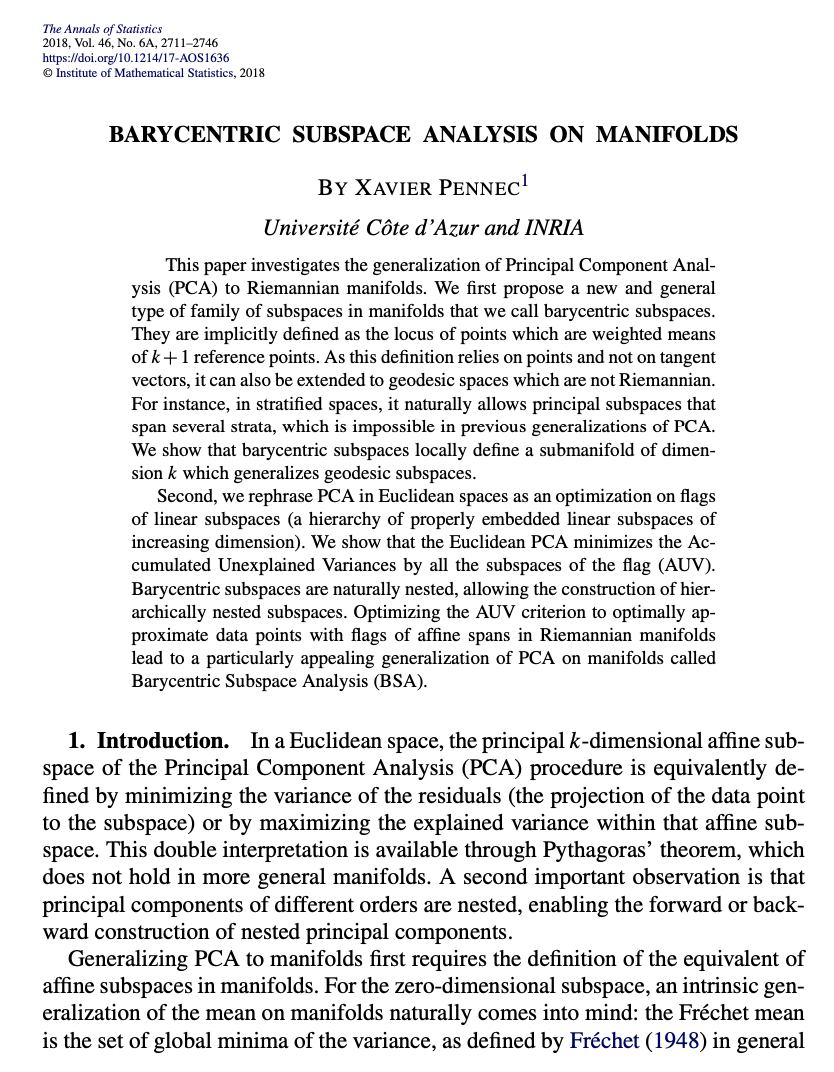
\includegraphics[width=0.8\linewidth]{figs/pennec2018-page1.png}}
\caption{% 
Primeira página do artigo sendo revisado. Para baixar, foi necessario o Scihub
pois o portal da CAPES nao continha este periodico apos 2017.
}\label{fig:paper:page1}
\end{figure}

Será utilizada uma mistura de línguas nesta revisão, sendo o inglês preferido
sempre que possível. Sendo assim, não teremos o trabalho de traduzir do inglês
algumas construções básicas do \LaTeX\ como \emph{Theorem} ou
\emph{Definition}.


\section{Tabela de Notação}

This section has a summary of the notation used in the paper.

\section{Commented and Expanded Abstract}

Aqui devemos comentar o abstract. Neste caso, escolhemos por comentar
cada parágrafo. Nesta seção, devemos procurar usar linguagem e observações mais
gerais, como se fosse um resumo expandido. Abaixo segue um screen shot do primeiro paragrafo.

{
\vspace{1em}
\frame{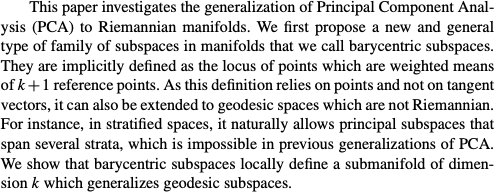
\includegraphics[width=0.8\linewidth]{figs/pennec2018-abstract-paragraph1.png}}
\vspace{1em}
}

Aqui o autor comenta que irá realizar uma extensão de PCA para Variedades
Riemannianas.

Variedades Riemannianas podem surgir, por exemplo, no contexto de \emph{data science}, de um conjunto de dados
provenientes de fenômenos não-lineares, em que os dados possuem uma estrutura de
similaridade ou métrica.

\todo{O que seria um espaço geodésico que não é Riemanniano?}

{
\vspace{1em}
\frame{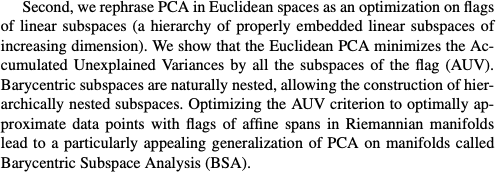
\includegraphics[width=0.8\linewidth]{figs/pennec2018-abstract-paragraph2.png}}
\vspace{1em}
}

\section{Commented and Expanded Section 1: Introduction}

{
\vspace{1em}
\frame{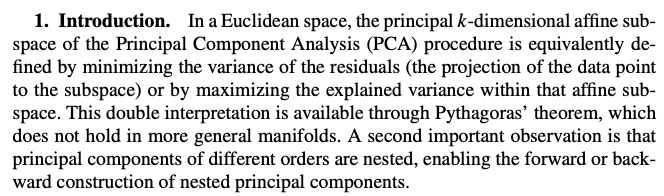
\includegraphics[width=0.8\linewidth]{figs/pennec2018-p1-paragraph1-intro.png}}
\vspace{1em}
}

Em poucas palavras, o PCA em espaços lineares (afim) pode ser definido
como o menor sub-espaço afim ($\mathbb R^n$ transladado) que contém os dados;
caso uma dimensão $n$ seja especificada, então o PCA de um conjunto é 
o menor sub-espaço afim de dimensão $k$ que capture a máxima variância dos dados
com $k$ dimensões. Se $k$ for maior que a dimensão do espaço que contém os dados
sem erro, então o PCA pode ser calculado sem perda. Se $k$ for menor que esse
valor, então o PCA vai conter perda. Conforme sabemos de Variedades
Diferenciáveis, muitos conjuntos de dados amostrados de fenômenos não-lineares,
por exemplo os provenientes de variedades diferenciáveis ou \emph{manifolds},
não são descritíveis globalmente por um único sistema de coordenadas de dimensão
míninima ou intrínseca. Logo, o PCA na maioria dos casos não-lineares incorre no
problema de ineficiência, pois muitos fenômenos não-lineares de forma global
com um único sistema de coordenadas cartesiano.

\emph{(Aqui vou escrever em ingles pra usar os jargões)}
PCA being ``nested'' means that the PCA subspace of dimension $k$ contains the
PCA subspace of dimension $k-1$. That is, the dimensions of the PCA are ordered,
so that if PCA has dimension $n$ then the lower dimensional subspaces that are
``best fit'' for the data are simply the same PCA subspace, but with the lower
dimension removed (the dimension along which the data has least variance). 
 


{
\vspace{1em}
\frame{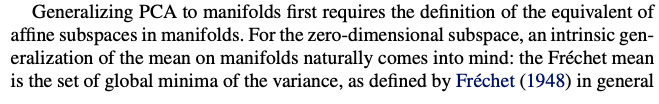
\includegraphics[width=0.8\linewidth]{figs/pennec2018-p1-paragraph2-intro.png}}
\vspace{1em}
}
\draftnote{Revisar aqui o conceito de Fréchet e também rapidamente o Karcher mean}


\section{Commented and Expanded Section 2: Riemannian geometry}

\section{Commented and Expanded Section 3: Exponential Barycentric Subspaces
(EBS) and affine spans}

\section{Commented and Expanded Section 4: Fréchet/Karcher barycentric
subspaces}


{
\vspace{1em}
\frame{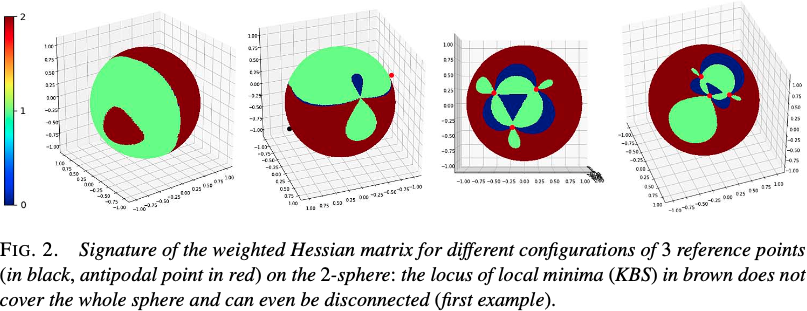
\includegraphics[width=0.8\linewidth]{figs/pennec2018-p18-fig2.png}}
\vspace{1em}
}

\todo{explicar cada figura do paper com proprias palavras e de forma expandida}

\section{Commented and Expanded Section 5: Properties of the barycentric
subspaces}

\section{Commented and Expanded Section 6: Barycentric subspace analysis}

\section{Commented and Expanded Section 7: Discussion}

\section{Commented and Expanded Appendix: Proof of Theorem 8}

\section{Commented and Expanded Supplementary Material}


\bibliographystyle{ieeetr}
\bibliography{refs}
%bib/edge-linking,bib/deformable,bib/medical,bib/graphics,bib/texture,bib/imaging,bib/tracking,bib/shape-papers,bib/bib-header,bib/video,bib/math-books,bib/math,bib/psych-books,bib/metric,bib/edge,bib/leymarie_pami_scaffold,bib/vision-books,bib/vision,bib/nn-search,bib/multidimscaling,bib/psychophysics,bib/indexing,bib/segmentation,bib/image-databases,bib/shape-matching,bib/neuro,bib/skeleton,bib/skeleton2D,bib/aspect-graphs,bib/recognition,bib/surface-networks,bib/ridge,bib/proceedings,bib/perceptual-grouping,bib/continuation,bib/graph-matching-2,bib/cooper}
%\input{paper.bbl}

% Assinaturas:
%\newpage
%\ \\\vspace{7cm}
%\center $\overline{\ \ \ Ricardo\ Fabbri\ \ \ }$
%\ \\\vspace{4cm}
%\center $\overline{\ \ \ Luciano\ da\ Fontoura\ Costa\ \ \ }$
\end{document}
